%% ----------------------------------------------------------------
%% Thesis.tex -- MAIN FILE (the one that you compile with LaTeX)
%% ---------------------------------------------------------------- 

% Set up the document
\documentclass[a4paper, 11pt, oneside]{Relatorio}  % Use the "Relatorio" style, based on the ECS Thesis style by Steve Gunn
\graphicspath{{Figure/}}  % Location of the graphics files (set up for graphics to be in PDF format)


% Include any extra LaTeX packages required
\usepackage[utf8]{inputenc}
\usepackage[brazilian]{babel}
\usepackage[T1]{fontenc}
\usepackage{ae,aecompl}
\usepackage{tabularx}
\usepackage[square, numbers, comma, sort&compress]{natbib}  % Use the "Natbib" style for the references in the Bibliography
\usepackage{verbatim}  % Needed for the "comment" environment to make LaTeX comments
%\usepackage{vector}  % Allows "\bvec{}" and "\buvec{}" for "blackboard" style bold vectors in maths
%\usepackage{listings}
\usepackage{listingsutf8}
\lstset{frame=tb,
  language=Python,
  aboveskip=3mm,
  belowskip=3mm,
  showstringspaces=false,
  columns=flexible,
  basicstyle={\small\ttfamily},
  numbers=none,
  numberstyle=\tiny\color{gray},
  keywordstyle=\color{dkblue},
  commentstyle=\color{dkgreen},
  stringstyle=\color{mauve},
  breaklines=true,
  breakatwhitespace=true,
  tabsize=4,
  lineskip={-1.5pt},
  morekeywords={models, lambda, forms, =}
  inputencoding=utf8,
  extendedchars=\true
}

\lstnewenvironment{code}[1][]%
  {\minipage{\linewidth}
   \lstset{basicstyle=\ttfamily\footnotesize,frame=tb,keepspaces=true,#1}}
  {\endminipage}


%%%% Color definitions
\usepackage{color}
\definecolor{dkgreen}{rgb}{0,0.6,0}
\definecolor{dkblue}{rgb}{0,0,0.5}
\definecolor{gray}{rgb}{0.5,0.5,0.5}
\definecolor{mauve}{rgb}{0.6,0,0.82}
\definecolor{coolblack}{rgb}{0.0, 0.18, 0.39}
\hypersetup{urlcolor=coolblack, colorlinks=true}  % Colours hyperlinks in blue, but this can be distracting if there are many links.
%\hypersetup{urlcolor=black, colorlinks=false}  

%% To show a border around all figures
%\usepackage{float}
%\floatstyle{boxed} 
%\restylefloat{figure}

%% ----------------------------------------------------------------
\begin{document}
\frontmatter	  % Begin Roman style (i, ii, iii, iv...) page numbering

% Set up the Title Page
\title  {Baobáxia}

\authors  {\texorpdfstring
            {\href{mailto:vince@mocambos.net}{Vincenzo Tozzi}} - 
            {\href{mailto:fernao@riseup.net}{Fernão Lopes}}
            }
\addresses  {\taina\\\npdd\\\redemocambos}  % Do not change this here, instead these must be set in the "Thesis.cls" file, please look through it instead
\date       {\today}
\subject    {Relatório de execução do projeto}
\keywords   {Federated Network, Tecnological Autonomy, Free Software, Rede Mocambos, Casa de Cultura Taina, Quilombo}

\maketitle
%% ----------------------------------------------------------------

\setstretch{1.3}  % It is better to have smaller font and larger line spacing than the other way round

% Define the page headers using the FancyHdr package and set up for one-sided printing
\fancyhead{}  % Clears all page headers and footers
\rhead{\thepage}  % Sets the right side header to show the page number
\lhead{}  % Clears the left side page header

\pagestyle{fancy}  % Finally, use the "fancy" page style to implement the FancyHdr headers

% %% ----------------------------------------------------------------
% % Declaration Page required for the Thesis, your institution may give you a different text to place here
% \Declaration{

% \addtocontents{toc}{\vspace{1em}}  % Add a gap in the Contents, for aesthetics

% Io, Vincenzo Tozzi, dichiaro che la presente tesi, "Reti federate eventualmente connesse" e il lavoro presentato in essa sono di mia paternità. Dichiaro che:

% \begin{itemize} 
% \item[\tiny{$\blacksquare$}] Questo lavoro è stato totalmente o per la maggior parte svolto come laureando per la Laurea in Informatica di questa Università.
 
% \item[\tiny{$\blacksquare$}] Ho esplicitamente dichiarato nel testo se qualche parte di questa tesi è stata precedentemente pubblicata in altri lavori da questa o altre Università o istituzioni.
 
% \item[\tiny{$\blacksquare$}] Ho attribuito la paternità ai lavori pubblicati da altri e da me consultati.
 
% \item[\tiny{$\blacksquare$}] Ho sempre citato la fonte di opere altrui. Ad eccezione di tali citazioni, questa tesi è di mia paternità.
 
% \item[\tiny{$\blacksquare$}] Ho ringranziato tutte le principali fonti di supporto.
 
% \item[\tiny{$\blacksquare$}] Ho esplicitamente dichiarato del testo, in parti sviluppate assieme ad altri, qual'è il loro e il mio contributo.
% \\
% \end{itemize}
 
 
% Firmato:\\
% \rule[1em]{25em}{0.5pt}  % This prints a line for the signature
 
% Data:\\
% \rule[1em]{25em}{0.5pt}  % This prints a line to write the date
% }
% \clearpage  % Declaration ended, now start a new page

%% ----------------------------------------------------------------
% The "Funny Quote Page"
\pagestyle{empty}  % No headers or footers for the following pages

\null\vfill
% Now comes the "Funny Quote", written in italics
\textit{``Vamos fazer um mundo mais do nosso jeito...''}

\begin{flushright}
Zumbi dos Palmares
\end{flushright}

\vfill\vfill\vfill\vfill\vfill\vfill\null
\clearpage  % Funny Quote page ended, start a new page
%% ----------------------------------------------------------------

% The Abstract Page
\addtotoc{Resumo}  % Add the "Abstract" page entry to the Contents
\abstract{

\addtocontents{toc}{\vspace{1em}}  % Add a gap in the Contents, for aesthetics

O projeto Baobáxia trata da concepção, desenvolvimento e implementação
de uma arquitetura distribuída, voltada para a integração de redes
locais mesmo em localidades nas quais a conexão à internet seja
instável, lenta ou intermitente. Parte-se da experiência acumulada
pela Rede Mocambos, que trabalha com a integração de mais de duzentas
comunidades em todas as regiões do país através da apropriação de
tecnologias, identificando pontos críticos em que a precariedade do
acesso à internet se torna um impeditivo para a efetiva comunicação
entre essas comunidades. O projeto parte do pressuposto de que não
basta usar as tecnologias de informação já existentes - é preciso
moldar o próprio desenvolvimento dessas tecnologias, para que atendam
às demandas da sociedade. Para isso, adota como princípio básico e
metodologia de trabalho os fundamentos do software livre - tanto na 
gestão das equipes de trabalho quanto nas soluções tecnológicas que 
utilizará.
}

\clearpage  % Abstract ended, start a new page
%% ----------------------------------------------------------------

\setstretch{1.3}  % Reset the line-spacing to 1.3 for body text (if it has changed)

% The Acknowledgements page, for thanking everyone
%% \acknowledgements{
%% \addtocontents{toc}{\vspace{1em}}  % Add a gap in the Contents, for aesthetics

%% Um agradecimento especial para as nossas familias\ldots

%% }
\clearpage  % End of the Acknowledgements
%% ----------------------------------------------------------------

\pagestyle{fancy}  %The page style headers have been "empty" all this time, now use the "fancy" headers as defined before to bring them back


%% ----------------------------------------------------------------
\lhead{\emph{Contents}}  % Set the left side page header to "Contents"
\tableofcontents  % Write out the Table of Contents

%% ----------------------------------------------------------------
%\lhead{\emph{List of Figures}}  % Set the left side page header to "List if Figures"
%\listoffigures  % Write out the List of Figures

%% ----------------------------------------------------------------
%\lhead{\emph{List of Tables}}  % Set the left side page header to "List of Tables"
%\listoftables  % Write out the List of Tables

%% ----------------------------------------------------------------
\setstretch{1.5}  % Set the line spacing to 1.5, this makes the following tables easier to read
\clearpage  % Start a new page
\lhead{\emph{Acrónimos}}  % Set the left side page header to "Abbreviations"
\listofsymbols{ll}  % Include a list of Abbreviations (a table of two columns)
{
% \textbf{Acronym} & \textbf{W}hat (it) \textbf{S}tands \textbf{F}or \\
  \textbf{RM} & \textbf{R}ede \textbf{M}ocambos\\ \textbf{SP} &
  \textbf{S}ervice \textbf{P}rovider\\ \textbf{IdP} &
  \textbf{Id}entity \textbf{P}rovider\\ \textbf{API} &
  \textbf{A}pplication \textbf{P}rogramming
  \textbf{I}nterface\\ \textbf{RFC} & \textbf{R}equest \textbf{F}or
  \textbf{C}omments\\ \textbf{JSON} & \textbf{J}ava\textbf{S}cript
  \textbf{O}bject \textbf{N}otation\\ \textbf{P2P} & \textbf{P}eer To
  \textbf{P}eer\\ \textbf{LDAP} & \textbf{L}ightweight
  \textbf{D}irectory \textbf{A}ccess \textbf{P}rotocol\\ \textbf{YAML}
  & \textbf{Y}et \textbf{A}nother \textbf{M}arkup
  \textbf{L}anguage\\ \textbf{XMPP} & e\textbf{X}tensible
  \textbf{M}essaging and \textbf{P}resence
  \textbf{P}rotocol\\ \textbf{SSO} & \textbf{S}ingle \textbf{S}ign
  \textbf{O}n\\ \textbf{VSAT} & \textbf{V}ery \textbf{S}mall
  \textbf{A}perture \textbf{T}erminal\\ \textbf{DRY} & \textbf{D}on't
  \textbf{R}epeat \textbf{Y}ourself\\ \textbf{MVC} & \textbf{M}odel
  \textbf{V}iew \textbf{C}ontroller\\ \textbf{ORM} & \textbf{O}bject
  \textbf{R}elational \textbf{M}apper\\ \textbf{NPDD} &
  \textbf{N}úcleo de \textbf{P}esquisa e \textbf{D}esenvolvimento
  \textbf{D}igital\\ \textbf{NFC} & \textbf{N}úcleo de
  \textbf{F}ormação \textbf{C}ontinuada\\ \textbf{NCP} &
  \textbf{N}úcleo de \textbf{C}omunicação e
  \textbf{P}edagogia\\ \textbf{GESAC} & \textbf{G}overno
  \textbf{E}letrônico \textbf{S}erviço de \textbf{A}tendimento ao
  \textbf{C}idadão\\ }

%% ----------------------------------------------------------------
%\clearpage  % Start a new page
%\lhead{\emph{Physical Constants}}  % Set the left side page header to "Physical Constants"
%\listofconstants{lrcl}  % Include a list of Physical Constants (a four column table)
%{
%% Constant Name & Symbol & = & Constant Value (with units) \\
%Speed of Light & $c$ & $=$ & $2.997\ 924\ 58\times10^{8}\ \mbox{ms}^{-\mbox{s}}$ (exact)\\
%
%}

%% ----------------------------------------------------------------
%\clearpage  %Start a new page
%\lhead{\emph{Simboli}}  % Set the left side page header to "Symbols"
%\listofnomenclature{lll}  % Include a list of Symbols (a three column table)
%{
%% symbol & name & unit \\
%$a$ & distance & m \\
%$P$ & power & W (Js$^{-1}$) \\
%& & \\ % Gap to separate the Roman symbols from the Greek
%$\omega$ & angular frequency & rads$^{-1}$ \\
%}
%% ----------------------------------------------------------------
% End of the pre-able, contents and lists of things
% Begin the Dedication page

%% \setstretch{1.3}  % Return the line spacing back to 1.3

%% \pagestyle{empty}  % Page style needs to be empty for this page
%% \dedicatory{Para nossa Mãe\ldots}

%% \addtocontents{toc}{\vspace{2em}}  % Add a gap in the Contents, for aesthetics


%% ----------------------------------------------------------------
\mainmatter	  % Begin normal, numeric (1,2,3...) page numbering
\pagestyle{fancy}  % Return the page headers back to the "fancy" style

% Include the chapters of the thesis, as separate files
% Just uncomment the lines as you write the chapters

\chapter{NPDD}\label{NPDD}\lhead{\leftmark}
O Núcleo de Pesquisa e Desenvolvimento Digital, NPDD, envolve pessoas
com conhecimento técnicos de varias comunidade e realidades da Rede. O
NPDD é responsável pelo desenvolvimento e manutenção das ferramentas
digitais da Rede, cuidando atualmente dos portais (www.mocambos.net,
wiki.mocambos.net, mapa.mocambos.net, galeria.mocambos.net), das
contas email (@mocambos.net e @mocambos.org) e de criar documentação
de base sobre as ferramentas digitais.

\section{Informações}

\subsection{Endereços e contatos}
Para informações e contatos podem escrever ao seguinte email, nosso
principal canal de comunicação: \\ \url{suporte@mocambos.org}

Existe também uma lista de discussão do NPDD hospedada no riseup.net:
\\ \url{mocambos-npdd@lists.riseup.net}

\begin{tabular}{lll}

\parbox[t]{0.3\textwidth}{
        \textbf{Distrito Federal} \\
        Mercado Sul \\
        QSB 12/13 Loja 7 \\
        Taguatinga/DF \\
}
        &
\parbox[t]{0.3\textwidth}{
        \textbf{São Paulo} \\
        Casa de Cultura Tainã \\
        Rua Inhambú, 645 \\
        Campinas/SP \\
        Telefone: (19) 32282993 \\
}
        &
\parbox[t]{0.35\textwidth}{
        \textbf{Sicilia/Itália} \\
        BOCS \\
        Via Piersanti Mattarella, 8 \\
        Bagheria \\
}

\end{tabular}

\section{Consultorias}
\subsection{Dynamite}
A versão 0.1 do projeto que foca na questão de metadados, conforme
plano de trabalho aprovado, foi desenvolvida com a consultoria da
Associação Cultural Dynamite (nota fiscal 0001000).


\section{Metodologia}
O projeto é conduzido pelo NPDD (Núcleo de Pesquisa e Desenvolvimento
Digital da Rede Mocambos), em sinergia com os demais Núcleos (NCP de
Comunicação e Pedagogia, NFC de Formação Continuada). À equipe fixa de
desenvolvedores se soma a participação de colaboradores e
especialistas em diferentes áreas. Sob a coordenação do NPDD, o
desenvolvimento se da de forma distribuída, utilizando-se ferramentas
colaborativas via internet como git, wiki e irc. A metodologia de
desenvolvimento segue o modelo ``Agile'' que prevê o lançamento
frequente de código funcionante para avaliação contínua por parte dos
usuários finais, permitindo a correção e a melhoria ao longo do
trabalho.

\subsection{Wiki}
A documentação do projeto é disponível no wiki da Rede Mocambos no
endereço: \\ \url{http://wiki.mocambos.net/NPDD/Baobáxia}

\subsection{Codigo}
O codigo do projeto é disponível em licença GPLv3 no Github no
endereço: \\ \url{http://github.com/RedeMocambos/baobaxia}

\subsection{Necessidades/Issues}
As necessidades do projeto são registradas no sistema de issues do
github no endereço:
\\ \url{http://github.com/RedeMocambos/baobaxia/issues}

 % NPDD
\chapter{Metadados}\label{Metadados}\lhead{\leftmark}

\section{Descrição geral da pesquisa de Metadados e políticas de metadados}
A pesquisa sobre metadados para o sistema Baobáxia compreendeu as
definições diretamente relacionadas aos metadados das mídias e também
a participação na modelagem geral dos objetos do sistema, assim como a
definição de formatos para troca de dados. Por metadados entendemos
toda a informação a respeito de si, seja para a mídia, seja para as
Mucuas como para o sistema. Deste modo, num entendimento amplo de
metadados, consideramos que qualquer dado descritivo a respeito do
sistema como um todo deve ser entendido como um metadado, e logo deve
ser armazenado em arquivos de definição.

Essa diretiva partiu de uma orientação em conjunto com o
desenvolvimento do núcleo do software Baobáxia
(https://github.com/RedeMocambos/baobaxia). Deste modo, tudo que
envolve a descrição de elementos do sistema pode ser considerado um
metadado. Os metadados, embora tenham como objetivo a estabilidade da
informação, devem contemplar a possibilidade de alterações nas suas
definições, bem como a expansão futura.

De início, definem-se dois tipos principais de metadado:
\begin{itemize}
\item metadado do sistema / políticas (arquivos de configuração,
  regras de funcionamento)
\item metadado do acervo/das mídias
\end{itemize}

Não coube à pesquisa em metadados a definição das políticas, mas a
orientação de como estas deveriam ser armazenadas e estruturadas. As
políticas de sistema dizem respeito a definições gerais sobre a
configuração do software e de critérios estabelecidos politicamente,
isto é, atendendo às demandas da comunidade usuária e gestora do
sistema Baobáxia. Entretanto, há uma escolha que entende a importância
da distinção entre o sistema e suas configurações, estas que devem ser
implementadas de acordo com as necessidades locais da Mucua ou do
repositório (baobáxia / Rede Mocambos).

A partir da definição de políticas, ocorre a tomada de decisões pelo
sistema, respeitando aos critérios estabelecidos. Essa definição
possui normas técnicas próprias, mas é abrangente o bastante para
permitir que novas políticas sejam incorporadas ao sistema conforme
surjam novas necessidades.

\section{Mídias e Mucuas}
Os metadados relacionados a mídias e mucuas constituem o núcleo do
sistema. Em tratando-se de um sistema de acervo distribuído, os nós
(Mucuas) e arquivos contidos nesses nós (Mídias) são os principais
elementos do sistema do ponto de vista dos conteúdos.

As mídias sempre estão associadas a mucuas originadoras (as quais originaram a publicação), e dividem-se por tipos:
\begin{itemize}
\item vídeos
\item imagens (fotografias, desenhos etc)
\item áudios (músicas, entrevistas, programas de rádio etc)
\item arquivos (documentos, textos e demais arquivos)
\end{itemize}

Cada tipo de mídia possui especificidades do ponto de vista de seus
metadados, ao que buscou-se definir o que há de comum entre todas. Os
metadados foram definidos preliminarmente como o mínimo essencial
possível, sendo que qualificadores adicionais devem ser estendidos ou
como tags ou como metadados específicos do tipo de arquivo. Assim,
chegou-se aos seguintes campos, cuja definição encontra-se nos
arquivos de políticas (ver adiante):
\begin{itemize}
\item data (AAAA-MM-DD)
\item uuid (identificação única do arquivo)
\item title (título, texto não único)
\item comment (comentário, texto aberto)
\item author (mocambola, associado a quem publicou o arquivo)
\item type (tipos das mídias [vídeo|imagens|áudios|arquivos])
\item format (formato do arquivo, definido em arquivo de políticas)
\item origin (mucua, o servidor a partir do qual arquivo foi
  publicado)
\item repository (referência ao repositório git annex a que está vinculado o arquivo)
\item tags (etiquetas, múltiplas; somente descritoras ou também
  funcionais)
\end{itemize}

Além da mídia, as mucuas (nós do acervo, servidores locais) possuem
também metadados específicos, bem como associados. Os metadados
específicos dizem respeito a informações ligadas diretamente ao
servidor; as associadas, ao conteúdo hospedado no servidor. Dessa
forma, temos:
\begin{itemize}
\item note (texto geral sobre a mucua)
\item description (nome da mucua)
\item uuid (identificador único da mucua)
\end{itemize}


Quanto ao metadado associado, diz respeito a todas as etiquetas de
conteúdos que estejam hospedados na mucua. Está previsto como um
metadado descritivo sobre a mucua um relatório agrupando todas as
etiquetas dos arquivos hospedados, o que permite aos mocambolas
(usuári@s) terem uma ideia geral sobre as características do acervo
de determinada Mucua.

\section{Armazenamento do metadado: arquivos, padrões adotados e intercâmbio}
Conforme já assinalado, metadados e políticas são armazenados em
arquivos descritores. Para tal foi feita uma pesquisa a respeito dos
formatos a serem adotados para armazenamento destes dados. Teriam de
atender os seguintes requisitos:
\begin{description}
\item[A] armazenamento em suporte aberto, não proprietário
\item[B] ótima capacidade de intercâmbio entre linguagens
\item[C] amplo desenvolvimento de bibliotecas de código em distintas linguagens de programação
\item[D] capacidade para armazenamento de objetos complexos
\item[E] bom desempenho
\item[F] tamanho diminuto
\item[G] adequação a plataformas RESTful e serviços de dados (web services)
\end{description}

Inicialmente, levantou-se três possibilidades, todas elas atendendo os itens A e B:
\begin{description}
\item[XML] eXpansible Markup Language
\item[YAML] Yet Another Markup Languge
\item[JSON] JavaScript Object Notation
\end{description}

O primeiro formato, XML, tem a seu favor o fato de ser largamente
adotado para intercâmbio de dados e para descrição de informações já
há muitos anos (C). Conta no entanto com algumas desvantagens
sobretudo do ponto de vista do desempenho (E), além de gerar uma não
desprezível quantidade de informações extra especialmente ao lidar com
o armazenamento de objetos complexos, o que tem impactos severos ao se
pensar numa rede de acervos com conectividade baixa ou nula (ponto
F). Além disso, conta com possíveis problemas no armazenamento de
objetos complexos ao redundar numa estrutura de dados pesada (D).

O segundo formato, YAML, apresenta-se como um possível sucessor do
XML, tendo se inspirado neste. Tem como resultado arquivos sintéticos
e de tamanho diminuto (E e F). Possui ótima capacidade de
armazenamento de objetos complexos (D). Apesar de contar com mais
funcionalidades que o JSON - como a possibilidade de estabelecer
relacionamentos funcionais lógicos internos, conta ainda com menor
desenvolvimento e compatibilidade (C e G), ainda que seu futuro seja
promissor.

O terceiro formato, JSON, é considerado uma forma de reduzir o
overhead computacional do XML (E), sendo uma excelente alternativa
para armazenamento de objetos complexos (D), sendo sintético e de
tamanho diminuto (F). Conta com grande desenvolvimento em uma série de
softwares (C) pode-se dizer que atualmente é o novo padrão para
intercâmbio de dados, sendo base para numerosas tecnologias baseadas
em plataformas RESTful (G)

Desse modo, foi escolhido o formato JSON como padrão para intercâmbio
de dados, definição de políticas e metadados.

\section{Politicas}

\subsection{Media}

Definição dos metadados de mídia:
\begin{description}
  \item[formats] definem-se os tipos de formatos aceitos
  \item[priority] tipos prioritários aceitos pelo sistema
  \item[metadata] definição dos campos com tipo de dados aceito. Pode
    receber uma expressão regular (ex.: \verb| /^\w_-$/ |)
\end{description}

\lstinputlisting[basicstyle={\scriptsize\ttfamily}]{../../policies/media.json}

\subsection{Mucua}

\lstinputlisting[basicstyle={\scriptsize\ttfamily}]{../../policies/mucua.json}


 % Metadados
\chapter{Repositórios}\label{Repositórios}\lhead{\leftmark}

A arquitetura descentralizada do Baobáxia é baseada em repositórios
\emph{git} e \emph{git-annex}.

Um elemento importante para o acervo multimídia são as operações de
sincronização. As ferramentas baseadas no \emph{git} herdam a sua
natureza descentralizada e a capacidade de comunicar de forma
transparente usando vários protocolos. Em particular é interessante a
possibilidade de executar sincronizações com sistemas de armazenamento
massivo, característica essencial na fase de criação de um novo nó,
onde a primeira sincronização via rede poderia levar dias. As
transferências contudo, no caso do \emph{git-annex}, são executadas
através do protocolo \emph{rsync}\footnote{\emph{rsync} é um Software
  Livre para a transfêrencia rápida e incremental de arquivos
  disponível no \url{http://rsync.samba.org/}.}, que gerencia
eventuais interrupções, evitando retransmissões onerosas.


\subsection{Git}\label{sec:GIT}
Git é um sistema multiplataforma para o controle de versão
distribuído, projetado para ser rápido e usável mesmo em grande
projetos.

As características principais incluem:
\begin{itemize}
\item é totalmente distribuído e cada clone de um repositório contem o
  histórico inteiro das versões e no qual podem ser efetuadas
  operações independentemente de conexões de rede o de servidores
  centrais. As mudanças podem ser copiadas entre um clone e o outro e
  são mantidos em \emph{branch} (ramos) diferentes, facilitando as
  operações de \emph{merge} (fusão). Os repositórios são facilmente
  acessíveis através do eficiente protocolo do Git, que além de
  suportar HTTP, pode funcionar junto com SSH, para obter conexões
  seguras e um sistema de autenticação solido e bem comum.
\item suporta o \emph{branching} (ramificação), e o \emph{merging}
  (fusão), de maneira rápida e conveniente, incluindo uma serie de
  ferramentas para visualizar e navegar o histórico não linear das
  versões.
\item é muito rápido e escala mesmo em projetos muito grandes e com
  muitas mudanças, graças a um eficiente sistema de empacotamento e
  memorização do histórico (é considerado o mais eficiente entre os
  sistemas atualmente disponíveis).
\item associa um nome de versão, para cada \emph{commit}, que é função
  do histórico inteiro, por isso, uma vez publicada uma versão, não é
  possível alterar as velhas sem ser notado. As versões podem também
  ser etiquetadas e assinadas digitalmente com GPG.
\end{itemize}

Git é um sistema completo que, em bom estilo Unix, é organizado em
programas e comandos independentes, pensados para ser facilmente
usáveis, seja automaticamente através de \emph{scripting} seja de
maneira interativa pelo usuário final. Git é, então, uma base solida
para o desenvolvimento de aplicações orientadas a sincronização, a
portabilidade e a gestão autônoma e descentralizada. 

\subsection{git-annex}\label{git-annex}
\emph{git-annex}\footnote{\emph{git-annex} é um programa que estende
  as funcionalidades do \emph{git} em gerir arquivos de grande tamanho
disponível no \url{http://git-annex.branchable.com}.} permite a
gestão de arquivos com \emph{git}, sem a necessidade de adicionar os
arquivos dentro \emph{git}. Mesmo se pode parecer paradoxal, é útil
quando se trabalha com arquivos muito grandes que \emph{git}
atualmente não gerencia facilmente por limitações devidas a memoria,
tempo ou espaço no disco.

Mesmo sem manter o histórico das mudanças do conteúdo do arquivo, ter
a possibilidade de gerenciar arquivos com \emph{git}, de movê-los, e
exclui-los, numa árvore de pasta versionada, com uso de
\emph{branches} e de clones distribuídos, são todos bons motivos para
usar \emph{git}. E os arquivos anexos (por isso o nome
\emph{git-annex}) podem coexistir no mesmo repositório \emph{git} com
os arquivos regularmente versionados. 

\emph{git-annex} transforma os arquivos anexos em \emph{link}
simbólicos, que são normalmente versionados por \emph{git}. 

O conteúdo dos arquivos é mantido por \emph{git-annex} em um acervo
chave/valor distribuído que corresponde aos clones de um dado
repositório \emph{git}. Praticamente \emph{git-annex} memoriza o
conteúdo do arquivo em uma subpasta de \verb|.git/annex/|.

A primeira vez que um arquivo é adicionado no \emph{git-annex}, é
calculada uma chave, normalmente fazendo um \emph{hash} do seu
conteúdo. \emph{git-annex} todavia suporta vários \emph{backend} que
podem produzir diferentes tipos de chaves. O arquivo que é adicionado
no \emph{git} nada mais é que um \emph{link} simbólico para a chave
memorizada no \verb|.git/annex/|. Se o conteúdo do arquivo for
modificado, é gerada uma outra chave, e o \emph{link} é alterado. 

O conteúdo do arquivo pode ser transferido de um repositório para
outro por \emph{git-annex}, que além de manter controle de quem mantem
o que, permite criar um mapa das copias disponíveis e impor um número
mínimo de cópias. Essas informações são mantidas em um \emph{branch}
separado, chamado ``\emph{git-annex}'', e as operações de
sincronização, são simplesmente \emph{push} e \emph{pull} entre os
vários clones dos repositórios.

\emph{git-annex} suporta:
\begin{itemize}
\item localização das cópias (\emph{location tracking})
\item download seletivo dos conteúdos 
\item gestão da confiança dos repositórios
\item gestão do número minimo de cópias
\item vários \emph{backend} para as chaves (SHA\footnote{Secure Hash
    Algoritm, (SHA), é um algoritmo usado em sistemas chave/valor onde
    as chaves são calculadas através de uma função criptográfica dos
    valores.}, WORM\footnote{O algoritmo WORM identifica os arquivos
    em base ao nome, dimensão e data de alteração.})
\item vários \emph{backend} para os conteúdos/valores
  (BUP\footnote{BUP é um sistema para \emph{backup} a alta eficiência
    disponível no: \url{https://github.com/apenwarr/bup}.}, rsync,
  web, S3\footnote{Amazon Simple Storage Service, (S3) é uma
    infraestrutura para a memorização dos dados totalmente redundante,
    disponível no: \url{aws.amazon.com/}.})
\end{itemize}

\section{Gestão de repositórios multiplos}
A arquitetura baseadas em repositórios se adapta ao contexto de
``redes federadas'' onde para cada ``Rede'' corresponde um
repositório. A solução proposta no Baobáxia inclui já a possibilidade
de cadastrar e gerenciar varias redes. A associação rede/repositório
permite a escalabilidade da arquitetura e uma gestão diferenciada dos
conteúdos. Cada mucua pode se associar a diferentes redes, por
exemplo, Rede Mocambos, Estaçoes Digitais, etc.

\begin{figure}[htbp]
  \centering
  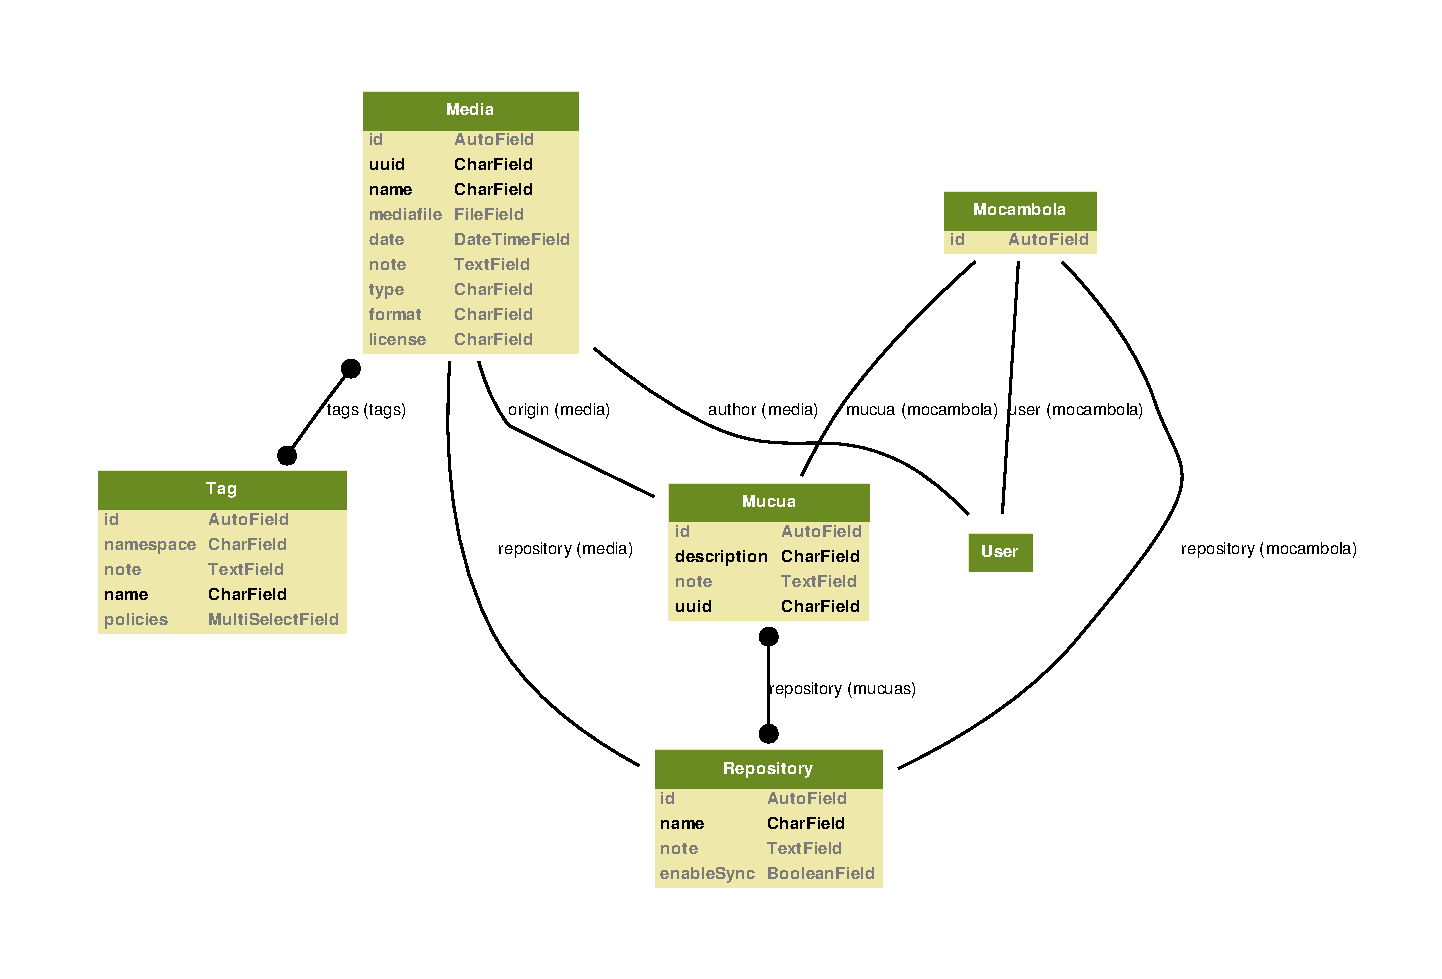
\includegraphics[width=\textwidth]{./Fig/Auto_UML_Diagram.pdf}
  \rule{35em}{0.5pt}
  \caption[Diagrama UML do BBX]{Diagrama UML do BBX}
  \label{fig:SchemaServer_ReteMocambos}
\end{figure}

\subsection{API e rotas}
A API REST proposta prevê a gestão de repositórios multiplos em
diferentes mucuas, usando o padrão de endereços:
$$ /repositorio/mucua/ $$ 

Por exemplo, para acessar um ``media'' (uuid
aa9f9019-e4f2-4040-bc46-c2e15b66bebc) publicado na ``Rede Mocambos'', na
mucua ``Dandara'' o endereço é:
$$ /mocambos/dandara/media/aa9f9019-e4f2-4040-bc46-c2e15b66bebc $$

ou no caso da ``Estaçao Digital'' na ``Samambaia'' seria:
$$ /fbb/samambaia/media/aa9f9019-e4f2-4040-bc46-c2e15b66bebc $$

O detalhamento da API e das rotas será definido em capitulo especifico. % REF.

\subsection{Autenticação}
O Baobáxia pode gerenciar dados de varias redes/organizações e
portanto precisa diferenciar os usuários por Rede e Mucua\footnote{A
  mucua de alguma forma identifica uma comunidade}. No caso as
credenciais dos usuários são mantidas em arquivos versionados pelo git
nos repositórios correspondentes.

Para manter compatibilidade com outras aplicações do django mantivemos
o User padrão do django usando somente o campo username para codificar
as informarções necessárias.

Um mocambola\footnote{Usuário} é definido por nome, mucua e
repositorio no padrão:
$$ nome@mucua.repositorio.tld $$ .

O django é muito flexivel e suporta diferentes sistemas de
autenticação, com a possibilidade de definir seu proprio backend
personalizado.

O backend de autenticação personalizado, ``FileBackend'' se encontra
em \emph{bbx/auth.py}.

No BBX, os usuários são serializados em formato \emph{json} e
armazenados seguindo o seguinte padrão de localização:
$$ /repositorio/mucua/mocambolas/usuario.json $$

Por exemplo, no caso do mocambola ``zumbi'' da Casa de Cultura
Tainã cuja mucua se chama ``dandara'':
$$ zumbi@dandara.mocambos.net $$
$$ /mocambos/dandara/mocambolas/zumbi@dandara.mocambos.net $$

Notar que o repositório não inclui a extensão de dominio de primeiro
nível, no caso do exemplo ``.net'', que permanece no username do
mocambola.


 % Multirepositorio
\chapter{Transferências e sincronização dos mídias}\label{Transferências e sincronização dos mídias}\lhead{\leftmark}

\section{Transferência agendada e seletiva de arquivos}
A arquitetura do \emph{git-annex} se baseia em clones do repositório
que sincronizam entre si os conteúdos. Pela especifica de requisitos
da RM é necessário que as operações de sincronização possam acontecer
em contextos offline. Nesses contextos os conteúdos de fato viagiam
fisicamente em suportes quais laptops, HDs e pendrive. O meio de
transporte dos dados é portanto baseado nas rotas fisicas da Rota dos
Baobás. As Rotas nascem de vinculos concretos ancestrais, de
afinidade, troca de produtos, encontros e vivencias, que já existem
entre as comunidades. O Baobáxia tenta aproveitar o maximo possível as
logicas e os vinculos preexistentes. Para entender melhor o
funcionamento detalhamos um pouco a Rota dos Baobás a partir da Tainã
que mantem relações constantes com:
\begin{itemize}
  \item Quilombo do Cafundó
  \item Fazenda Roseira
  \item Quilombo de Brotas
  \item Mercado Sul
\end{itemize}

A Tainã e o Mercado Sul dispõem de conexão em banda larga, a Roseira
esta sem conexão internet e o Cafundó tem uma conexão satelitar.

A base da logica de triagem e circulação dos conteúdos é gerenciada
atraves dos ``preferred contents'' do \emph{git-annex}, que
possibilita organizar as \emph{mucuas} por grupos e definir regras de
circulação entre esses grupos baseados em diferentes metadados (tipo
de arquivo, tag, tamanho, ...).

A rede do Baobáxia pode ser reconfigurada ``em andamento'', ou seja as
logica de triagem podem mudar no tempo. Escolhemos como primeira
configuração:

\begin{tabular}{ l | c || r }
  \hline                       
  nucleo & 3 & taina, mercado sul \\
  sync & 2 & raspberry, laptop \\
  online & 2 & acotirene,  \\
  \hline  
\end{tabular}




\section{Gestão de conflitos entre versões}

%% A arquitetura descentralizada do Baobáxia é baseada em repositórios
%% \emph{git} e \emph{git-annex}.

%% Um elemento importante para o acervo multimídia são as operações de
%% sincronização. As ferramentas baseadas no \emph{git} herdam a sua
%% natureza descentralizada e a capacidade de comunicar de forma
%% transparente usando vários protocolos. Em particular é interessante a
%% possibilidade de executar sincronizações com sistemas de armazenamento
%% massivo, característica essencial na fase de criação de um novo nó,
%% onde a primeira sincronização via rede poderia levar dias. As
%% transferências contudo, no caso do \emph{git-annex}, são executadas
%% através do protocolo \emph{rsync}\footnote{\emph{rsync} é um Software
%%   Livre para a transfêrencia rápida e incremental de arquivos
%%   disponível no \url{http://rsync.samba.org/}.}, que gerencia
%% eventuais interrupções, evitando retransmissões onerosas.


%% \subsection{Git}\label{sec:GIT}
%% Git é um sistema multiplataforma para o controle de versão
%% distribuído, projetado para ser rápido e usável mesmo em grande
%% projetos.

%% As características principais incluem:
%% \begin{itemize}
%% \item é totalmente distribuído e cada clone de um repositório contem o
%%   histórico inteiro das versões e no qual podem ser efetuadas
%%   operações independentemente de conexões de rede o de servidores
%%   centrais. As mudanças podem ser copiadas entre um clone e o outro e
%%   são mantidos em \emph{branch} (ramos) diferentes, facilitando as
%%   operações de \emph{merge} (fusão). Os repositórios são facilmente
%%   acessíveis através do eficiente protocolo do Git, que além de
%%   suportar HTTP, pode funcionar junto com SSH, para obter conexões
%%   seguras e um sistema de autenticação solido e bem comum.
%% \item suporta o \emph{branching} (ramificação), e o \emph{merging}
%%   (fusão), de maneira rápida e conveniente, incluindo uma serie de
%%   ferramentas para visualizar e navegar o histórico não linear das
%%   versões.
%% \item é muito rápido e escala mesmo em projetos muito grandes e com
%%   muitas mudanças, graças a um eficiente sistema de empacotamento e
%%   memorização do histórico (é considerado o mais eficiente entre os
%%   sistemas atualmente disponíveis).
%% \item associa um nome de versão, para cada \emph{commit}, que é função
%%   do histórico inteiro, por isso, uma vez publicada uma versão, não é
%%   possível alterar as velhas sem ser notado. As versões podem também
%%   ser etiquetadas e assinadas digitalmente com GPG.
%% \end{itemize}

%% Git é um sistema completo que, em bom estilo Unix, é organizado em
%% programas e comandos independentes, pensados para ser facilmente
%% usáveis, seja automaticamente através de \emph{scripting} seja de
%% maneira interativa pelo usuário final. Git é, então, uma base solida
%% para o desenvolvimento de aplicações orientadas a sincronização, a
%% portabilidade e a gestão autônoma e descentralizada. 

%% \subsection{git-annex}\label{git-annex}
%% \emph{git-annex}\footnote{\emph{git-annex} é um programa que estende
%%   as funcionalidades do \emph{git} em gerir arquivos de grande tamanho
%% disponível no \url{http://git-annex.branchable.com}.} permite a
%% gestão de arquivos com \emph{git}, sem a necessidade de adicionar os
%% arquivos dentro \emph{git}. Mesmo se pode parecer paradoxal, é útil
%% quando se trabalha com arquivos muito grandes que \emph{git}
%% atualmente não gerencia facilmente por limitações devidas a memoria,
%% tempo ou espaço no disco.

%% Mesmo sem manter o histórico das mudanças do conteúdo do arquivo, ter
%% a possibilidade de gerenciar arquivos com \emph{git}, de movê-los, e
%% exclui-los, numa árvore de pasta versionada, com uso de
%% \emph{branches} e de clones distribuídos, são todos bons motivos para
%% usar \emph{git}. E os arquivos anexos (por isso o nome
%% \emph{git-annex}) podem coexistir no mesmo repositório \emph{git} com
%% os arquivos regularmente versionados. 

%% \emph{git-annex} transforma os arquivos anexos em \emph{link}
%% simbólicos, que são normalmente versionados por \emph{git}. 

%% O conteúdo dos arquivos é mantido por \emph{git-annex} em um acervo
%% chave/valor distribuído que corresponde aos clones de um dado
%% repositório \emph{git}. Praticamente \emph{git-annex} memoriza o
%% conteúdo do arquivo em uma subpasta de \verb|.git/annex/|.

%% A primeira vez que um arquivo é adicionado no \emph{git-annex}, é
%% calculada uma chave, normalmente fazendo um \emph{hash} do seu
%% conteúdo. \emph{git-annex} todavia suporta vários \emph{backend} que
%% podem produzir diferentes tipos de chaves. O arquivo que é adicionado
%% no \emph{git} nada mais é que um \emph{link} simbólico para a chave
%% memorizada no \verb|.git/annex/|. Se o conteúdo do arquivo for
%% modificado, é gerada uma outra chave, e o \emph{link} é alterado. 

%% O conteúdo do arquivo pode ser transferido de um repositório para
%% outro por \emph{git-annex}, que além de manter controle de quem mantem
%% o que, permite criar um mapa das copias disponíveis e impor um número
%% mínimo de cópias. Essas informações são mantidas em um \emph{branch}
%% separado, chamado ``\emph{git-annex}'', e as operações de
%% sincronização, são simplesmente \emph{push} e \emph{pull} entre os
%% vários clones dos repositórios.

%% \emph{git-annex} suporta:
%% \begin{itemize}
%% \item localização das cópias (\emph{location tracking})
%% \item download seletivo dos conteúdos 
%% \item gestão da confiança dos repositórios
%% \item gestão do número minimo de cópias
%% \item vários \emph{backend} para as chaves (SHA\footnote{Secure Hash
%%     Algoritm, (SHA), é um algoritmo usado em sistemas chave/valor onde
%%     as chaves são calculadas através de uma função criptográfica dos
%%     valores.}, WORM\footnote{O algoritmo WORM identifica os arquivos
%%     em base ao nome, dimensão e data de alteração.})
%% \item vários \emph{backend} para os conteúdos/valores
%%   (BUP\footnote{BUP é um sistema para \emph{backup} a alta eficiência
%%     disponível no: \url{https://github.com/apenwarr/bup}.}, rsync,
%%   web, S3\footnote{Amazon Simple Storage Service, (S3) é uma
%%     infraestrutura para a memorização dos dados totalmente redundante,
%%     disponível no: \url{aws.amazon.com/}.})
%% \end{itemize}

%% \section{Gestão de repositórios multiplos}
%% A arquitetura baseadas em repositórios se adapta ao contexto de
%% ``redes federadas'' onde para cada ``Rede'' corresponde um
%% repositório. A solução proposta no Baobáxia inclui já a possibilidade
%% de cadastrar e gerenciar varias redes. A associação rede/repositório
%% permite a escalabilidade da arquitetura e uma gestão diferenciada dos
%% conteúdos. Cada mucua pode se associar a diferentes redes, por
%% exemplo, Rede Mocambos, Estaçoes Digitais, etc.

%% \begin{figure}[htbp]
%%   \centering
%%   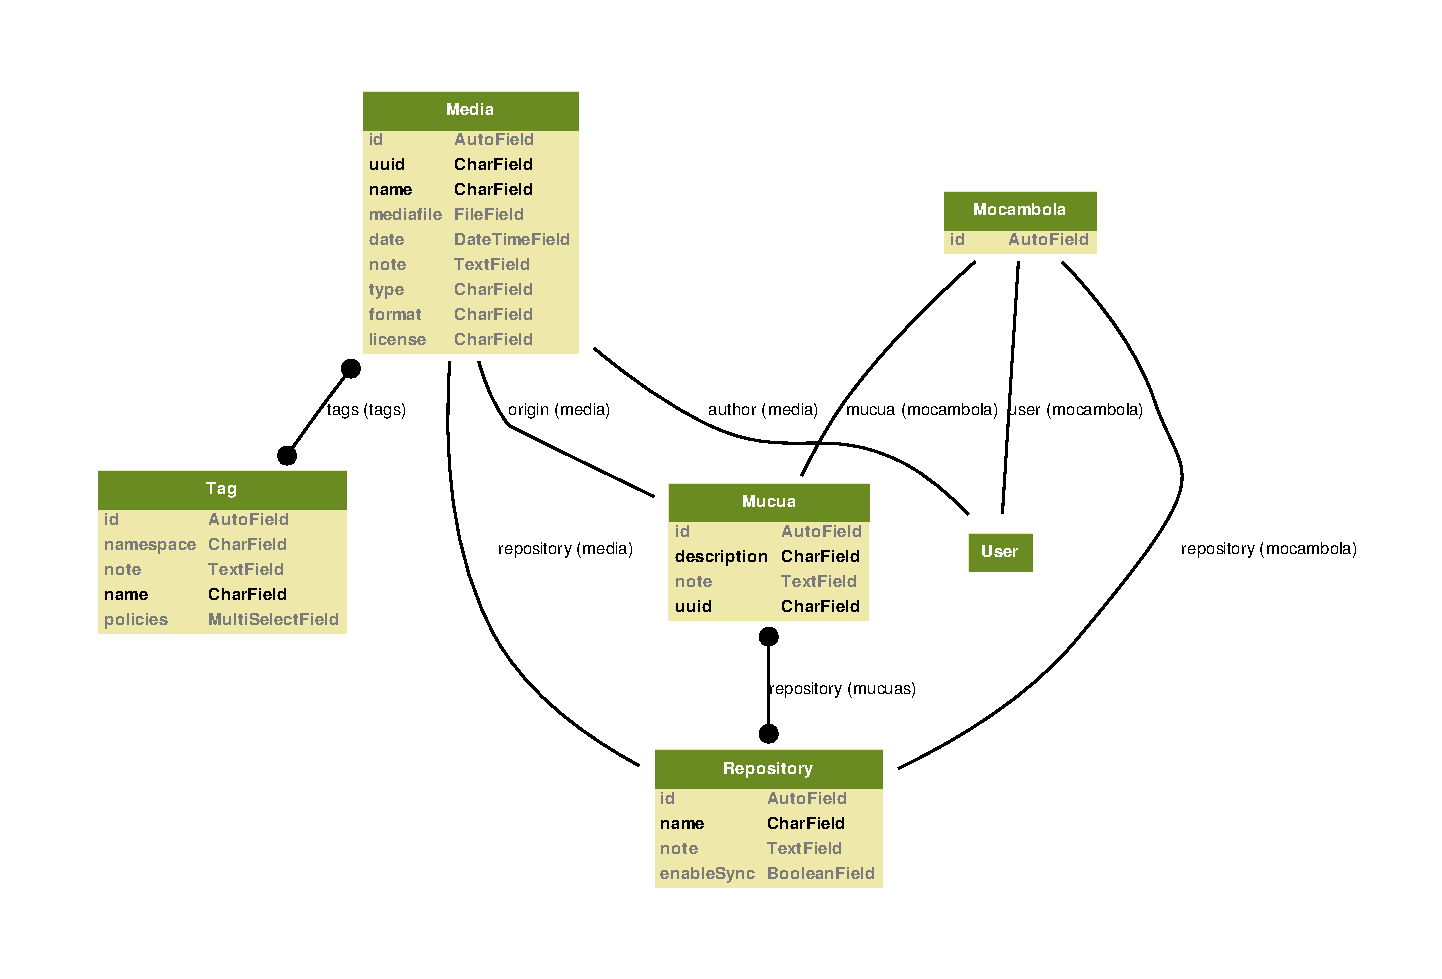
\includegraphics[width=\textwidth]{./Fig/Auto_UML_Diagram.pdf}
%%   \rule{35em}{0.5pt}
%%   \caption[Diagrama UML do BBX]{Diagrama UML do BBX}
%%   \label{fig:SchemaServer_ReteMocambos}
%% \end{figure}

%% \subsection{API e rotas}
%% A API REST proposta prevê a gestão de repositórios multiplos em
%% diferentes mucuas, usando o padrão de endereços:
%% $$ /repositorio/mucua/ $$ 

%% Por exemplo, para acessar um ``media'' (uuid
%% aa9f9019-e4f2-4040-bc46-c2e15b66bebc) publicado na ``Rede Mocambos'', na
%% mucua ``Dandara'' o endereço é:
%% $$ /mocambos/dandara/media/aa9f9019-e4f2-4040-bc46-c2e15b66bebc $$

%% ou no caso da ``Estaçao Digital'' na ``Samambaia'' seria:
%% $$ /fbb/samambaia/media/aa9f9019-e4f2-4040-bc46-c2e15b66bebc $$

%% O detalhamento da API e das rotas será definido em capitulo especifico. % REF.

%% \subsection{Autenticação}
%% O Baobáxia pode gerenciar dados de varias redes/organizações e
%% portanto precisa diferenciar os usuários por Rede e Mucua\footnote{A
%%   mucua de alguma forma identifica uma comunidade}. No caso as
%% credenciais dos usuários são mantidas em arquivos versionados pelo git
%% nos repositórios correspondentes.

%% Para manter compatibilidade com outras aplicações do django mantivemos
%% o User padrão do django usando somente o campo username para codificar
%% as informarções necessárias.

%% Um mocambola\footnote{Usuário} é definido por nome, mucua e
%% repositorio no padrão:
%% $$ nome@mucua.repositorio.tld $$ .

%% O django é muito flexivel e suporta diferentes sistemas de
%% autenticação, com a possibilidade de definir seu proprio backend
%% personalizado.

%% O backend de autenticação personalizado, ``FileBackend'' se encontra
%% em \emph{bbx/auth.py}.

%% No BBX, os usuários são serializados em formato \emph{json} e
%% armazenados seguindo o seguinte padrão de localização:
%% $$ /repositorio/mucua/mocambolas/usuario.json $$

%% Por exemplo, no caso do mocambola ``zumbi'' da Casa de Cultura
%% Tainã cuja mucua se chama ``dandara'':
%% $$ zumbi@dandara.mocambos.net $$
%% $$ /mocambos/dandara/mocambolas/zumbi@dandara.mocambos.net $$

%% Notar que o repositório não inclui a extensão de dominio de primeiro
%% nível, no caso do exemplo ``.net'', que permanece no username do
%% mocambola.



 % Sincronizacao

%\input{./Capitoli/Capitolo1} % Introduzione

%\input{./Capitoli/Capitolo2} % Reti Federate  

\clearpage  % To start a new page

%% ----------------------------------------------------------------
% The "Funny Quote Page"
\pagestyle{empty}  % No headers or footers for the following pages

\null\vfill
% Now comes the "Funny Quote", written in italics
\textit{``A força da rede esta nos nós''}

\begin{flushright}
TC
\end{flushright}

\vfill\vfill\vfill\vfill\vfill\vfill\null
\clearpage  % Funny Quote page ended, start a new page
%% ----------------------------------------------------------------

\pagestyle{fancy}  % Finally, use the "fancy" page style to implement
                   % the FancyHdr headers

%\input{./Capitoli/Capitolo4} % Prototipo

%\input{./Capitoli/Capitolo5} % Conclusioni

%\input{./Chapters/Chapter6} % Results and Discussion

%\input{./Chapters/Chapter7} % Conclusion

%% ----------------------------------------------------------------
% Now begin the Appendices, including them as separate files

\addtocontents{toc}{\vspace{2em}} % Add a gap in the Contents, for aesthetics

\appendix % Cue to tell LaTeX that the following 'chapters' are Appendices

% Apendice A                                                                                                                                                
\newcommand{\codeFolder}{../../tests/django-backbone_0}
                   
\chapter{Listagem do código}
\label{ApendiceA}
\lhead{Apêndice A \emph{Listagem do código}}

\section{bbx}

\subsection{bbx/auth.py}
\lstinputlisting[basicstyle={\scriptsize\ttfamily}]{\codeFolder/bbx/auth.py}

\subsection{bbx/utils.py}
\lstinputlisting[basicstyle={\scriptsize\ttfamily}]{\codeFolder/bbx/utils.py}

\section{media}

%\lstinputlisting[basicstyle={\scriptsize\ttfamily}]{\codeFolder/media/README}

%\subsection{media/admin.py}
%\lstinputlisting[basicstyle={\scriptsize\ttfamily}]{../../tests/django-backbone_0/media/admin.py}

\subsection{media/models.py}
\lstinputlisting[basicstyle={\scriptsize\ttfamily}]{\codeFolder/media/models.py}

\subsection{media/serializers.py}
\lstinputlisting[basicstyle={\scriptsize\ttfamily}]{\codeFolder/media/serializers.py}

\subsection{media/views.py}
\lstinputlisting[basicstyle={\scriptsize\ttfamily}]{\codeFolder/media/views.py}

\subsection{media/urls.py}
\lstinputlisting[basicstyle={\scriptsize\ttfamily}]{\codeFolder/media/urls.py}

%\subsection{media/urls.py}
%\lstinputlisting[basicstyle={\scriptsize\ttfamily}]{../../tests/django-backbone_0/media/urls.py}

%\subsection{media/management/commands/run scheduled jobs.py}
%\lstinputlisting[basicstyle={\scriptsize\ttfamily}]{../../tests/django-backbone_0/media/management/commands/run_scheduled_jobs.py}


\section{repository}

\lstinputlisting[basicstyle={\scriptsize\ttfamily}]{\codeFolder/repository/README}

%\subsection{repository/admin.py}
%\lstinputlisting[basicstyle={\scriptsize\ttfamily}]{../../tests/django-backbone_0/repository/admin.py}

\subsection{repository/models.py}
\lstinputlisting[basicstyle={\scriptsize\ttfamily}]{\codeFolder/repository/models.py}

\subsection{repository/signals.py}
\lstinputlisting[basicstyle={\scriptsize\ttfamily}]{\codeFolder/repository/signals.py}

\subsection{repository/management/commands/run scheduled jobs.py}
\lstinputlisting[basicstyle={\scriptsize\ttfamily}]{\codeFolder/repository/management/commands/run_scheduled_jobs.py}

%\subsection{repository/admin.py}
%\lstinputlisting[basicstyle={\scriptsize\ttfamily}]{\codeFolder/repository/admin.py}

\subsection{repository/serializers.py}
\lstinputlisting[basicstyle={\scriptsize\ttfamily}]{\codeFolder/repository/serializers.py}

\section{mucua}

\subsection{mucua/models.py}
\lstinputlisting[basicstyle={\scriptsize\ttfamily}]{\codeFolder/mucua/models.py}

\subsection{mucua/serializers.py}
\lstinputlisting[basicstyle={\scriptsize\ttfamily}]{\codeFolder/mucua/serializers.py}

\subsection{mucua/views.py}
\lstinputlisting[basicstyle={\scriptsize\ttfamily}]{\codeFolder/mucua/views.py}

%\subsection{mucua/signals.py}
%lstinputlisting[basicstyle={\scriptsize\ttfamily}]{\codeFolder/mucua/signals.py}

%\subsection{mucua/urls.py}
%\lstinputlisting[basicstyle={\scriptsize\ttfamily}]{\codeFolder/mucua/urls.py}

\section{mocambola}

\subsection{mocambola/models.py}
\lstinputlisting[basicstyle={\scriptsize\ttfamily}]{\codeFolder/mocambola/models.py}

%\subsection{mocambola/serializers.py}
%\lstinputlisting[basicstyle={\scriptsize\ttfamily}]{\codeFolder/mocambola/serializers.py}

\subsection{mocambola/views.py}
\lstinputlisting[basicstyle={\scriptsize\ttfamily}]{\codeFolder/mocambola/views.py}



\section{tag}

\subsection{tag/models.py}
\lstinputlisting[basicstyle={\scriptsize\ttfamily}]{\codeFolder/tag/models.py}

\subsection{tag/serializers.py}
\lstinputlisting[basicstyle={\scriptsize\ttfamily}]{\codeFolder/tag/serializers.py}

\subsection{tag/views.py}
\lstinputlisting[basicstyle={\scriptsize\ttfamily}]{\codeFolder/tag/views.py}

%\subsection{tag/signals.py}
%\lstinputlisting[basicstyle={\scriptsize\ttfamily}]{\codeFolder/tag/signals.py}

%\subsection{tag/urls.py}
%\lstinputlisting[basicstyle={\scriptsize\ttfamily}]{\codeFolder/tag/urls.py}


	% Appendice codice sorgente

%\input{./Appendices/AppendixB} % Appendix Title

%\input{./Appendices/AppendixC} % Appendix Title

\addtocontents{toc}{\vspace{2em}}  % Add a gap in the Contents, for aesthetics
\backmatter
\nocite{*}
%% ----------------------------------------------------------------
\label{Bibliography}
\lhead{\emph{Bibliografia}}  % Change the left side page header to "Bibliography"
\bibliographystyle{unsrtnat}  % Use the "unsrtnat" BibTeX style for formatting the Bibliography
\bibliography{Bibliography}  % The references (bibliography) information are stored in the file named "Bibliography.bib"

\end{document}  % The End
%% ----------------------------------------------------------------
